\documentclass[final,nocolorBG,a4,mobius,nototal,pdf,slideColor]{prosper}

\addtolength{\textheight}{-1cm}
\usepackage[T1]{fontenc}
\usepackage[latin1]{inputenc}
\pagestyle{plain}
\usepackage{amsmath}
\usepackage{graphicx}
\usepackage{amssymb}
\usepackage{alltt}
\usepackage{xspace}
\makeatletter

\newcommand{\textttbf}[1]{\texttt{\textbf{#1}}}

\input{colour.tex}

\usepackage{pstricks,pst-node,pst-text,pst-3d}
\usepackage{epsfig}

%\usepackage{colordvi}
\usepackage{epsf}

\message{<Paul Taylor's Proof Trees, 2 August 1996>}
%% Build proof tree for Natural Deduction, Sequent Calculus, etc.
%% WITH SHORTENING OF PROOF RULES!
%% Paul Taylor, begun 10 Oct 1989
%% *** THIS IS ONLY A PRELIMINARY VERSION AND THINGS MAY CHANGE! ***
%%
%% 2 Aug 1996: fixed \mscount and \proofdotnumber
%%
%%      \prooftree
%%              hyp1            produces:
%%              hyp2
%%              hyp3            hyp1    hyp2    hyp3
%%      \justifies              -------------------- rulename
%%              concl                   concl
%%      \thickness=0.08em
%%      \shiftright 2em
%%      \using
%%              rulename
%%      \endprooftree
%%
%% where the hypotheses may be similar structures or just formulae.
%%
%% To get a vertical string of dots instead of the proof rule, do
%%
%%      \prooftree                      which produces:
%%              [hyp]
%%      \using                                  [hyp]
%%              name                              .
%%      \proofdotseparation=1.2ex                 .name
%%      \proofdotnumber=4                         .
%%      \leadsto                                  .
%%              concl                           concl
%%      \endprooftree
%%
%% Within a prooftree, \[ and \] may be used instead of \prooftree and
%% \endprooftree; this is not permitted at the outer level because it
%% conflicts with LaTeX. Also,
%%      \Justifies
%% produces a double line. In LaTeX you can use \begin{prooftree} and
%% \end{prootree} at the outer level (however this will not work for the inner
%% levels, but in any case why would you want to be so verbose?).
%%
%% All of of the keywords except \prooftree and \endprooftree are optional
%% and may appear in any order. They may also be combined in \newcommand's
%% eg "\def\Cut{\using\sf cut\thickness.08em\justifies}" with the abbreviation
%% "\prooftree hyp1 hyp2 \Cut \concl \endprooftree". This is recommended and
%% some standard abbreviations will be found at the end of this file.
%%
%% \thickness specifies the breadth of the rule in any units, although
%% font-relative units such as "ex" or "em" are preferable.
%% It may optionally be followed by "=".
%% \proofrulebreadth=.08em or \setlength\proofrulebreadth{.08em} may also be
%% used either in place of \thickness or globally; the default is 0.04em.
%% \proofdotseparation and \proofdotnumber control the size of the
%% string of dots
%%
%% If proof trees and formulae are mixed, some explicit spacing is needed,
%% but don't put anything to the left of the left-most (or the right of
%% the right-most) hypothesis, or put it in braces, because this will cause
%% the indentation to be lost.
%%
%% By default the conclusion is centered wrt the left-most and right-most
%% immediate hypotheses (not their proofs); \shiftright or \shiftleft moves
%% it relative to this position. (Not sure about this specification or how
%% it should affect spreading of proof tree.)
%
% global assignments to dimensions seem to have the effect of stretching
% diagrams horizontally.
%
%%==========================================================================

\def\introrule{{\cal I}}\def\elimrule{{\cal E}}%%
\def\andintro{\using{\land}\introrule\justifies}%%
\def\impelim{\using{\Rightarrow}\elimrule\justifies}%%
\def\allintro{\using{\forall}\introrule\justifies}%%
\def\allelim{\using{\forall}\elimrule\justifies}%%
\def\falseelim{\using{\bot}\elimrule\justifies}%%
\def\existsintro{\using{\exists}\introrule\justifies}%%

%% #1 is meant to be 1 or 2 for the first or second formula
\def\andelim#1{\using{\land}#1\elimrule\justifies}%%
\def\orintro#1{\using{\lor}#1\introrule\justifies}%%

%% #1 is meant to be a label corresponding to the discharged hypothesis/es
\def\impintro#1{\using{\Rightarrow}\introrule_{#1}\justifies}%%
\def\orelim#1{\using{\lor}\elimrule_{#1}\justifies}%%
\def\existselim#1{\using{\exists}\elimrule_{#1}\justifies}

%%==========================================================================

\newdimen\proofrulebreadth \proofrulebreadth=.05em
\newdimen\proofdotseparation \proofdotseparation=1.25ex
\newdimen\proofrulebaseline \proofrulebaseline=2ex
\newcount\proofdotnumber \proofdotnumber=3
\let\then\relax
\def\hfi{\hskip0pt plus.0001fil}
\mathchardef\squigto="3A3B
%
% flag where we are
\newif\ifinsideprooftree\insideprooftreefalse
\newif\ifonleftofproofrule\onleftofproofrulefalse
\newif\ifproofdots\proofdotsfalse
\newif\ifdoubleproof\doubleprooffalse
\let\wereinproofbit\relax
%
% dimensions and boxes of bits
\newdimen\shortenproofleft
\newdimen\shortenproofright
\newdimen\proofbelowshift
\newbox\proofabove
\newbox\proofbelow
\newbox\proofrulename
%
% miscellaneous commands for setting values
\def\shiftproofbelow{\let\next\relax\afterassignment\setshiftproofbelow\dimen0 }
\def\shiftproofbelowneg{\def\next{\multiply\dimen0 by-1 }%
\afterassignment\setshiftproofbelow\dimen0 }
\def\setshiftproofbelow{\next\proofbelowshift=\dimen0 }
\def\setproofrulebreadth{\proofrulebreadth}

%=============================================================================
\def\prooftree{% NESTED ZERO (\ifonleftofproofrule)
%
% first find out whether we're at the left-hand end of a proof rule
\ifnum  \lastpenalty=1
\then   \unpenalty
\else   \onleftofproofrulefalse
\fi
%
% some space on left (except if we're on left, and no infinity for outermost)
\ifonleftofproofrule
\else   \ifinsideprooftree
        \then   \hskip.5em plus1fil
        \fi
\fi
%
% begin our proof tree environment
\bgroup% NESTED ONE (\proofbelow, \proofrulename, \proofabove,
%               \shortenproofleft, \shortenproofright, \proofrulebreadth)
\setbox\proofbelow=\hbox{}\setbox\proofrulename=\hbox{}%
\let\justifies\proofover\let\leadsto\proofoverdots\let\Justifies\proofoverdbl
\let\using\proofusing\let\[\prooftree
\ifinsideprooftree\let\]\endprooftree\fi
\proofdotsfalse\doubleprooffalse
\let\thickness\setproofrulebreadth
\let\shiftright\shiftproofbelow \let\shift\shiftproofbelow
\let\shiftleft\shiftproofbelowneg
\let\ifwasinsideprooftree\ifinsideprooftree
\insideprooftreetrue
%
% now begin to set the top of the rule (definitions local to it)
\setbox\proofabove=\hbox\bgroup$\displaystyle % NESTED TWO
\let\wereinproofbit\prooftree
%
% these local variables will be copied out:
\shortenproofleft=0pt \shortenproofright=0pt \proofbelowshift=0pt
%
% flags to enable inner proof tree to detect if on left:
\onleftofproofruletrue\penalty1
}

%=============================================================================
% end whatever box and copy crucial values out of it
\def\eproofbit{% NESTED TWO
%
% various hacks applicable to hypothesis list 
\ifx    \wereinproofbit\prooftree
\then   \ifcase \lastpenalty
        \then   \shortenproofright=0pt  % 0: some other object, no indentation
        \or     \unpenalty\hfil         % 1: empty hypotheses, just glue
        \or     \unpenalty\unskip       % 2: just had a tree, remove glue
        \else   \shortenproofright=0pt  % eh?
        \fi
\fi
%
% pass out crucial values from scope
\global\dimen0=\shortenproofleft
\global\dimen1=\shortenproofright
\global\dimen2=\proofrulebreadth
\global\dimen3=\proofbelowshift
\global\dimen4=\proofdotseparation
\global\count255=\proofdotnumber
%
% end the box
$\egroup  % NESTED ONE
%
% restore the values
\shortenproofleft=\dimen0
\shortenproofright=\dimen1
\proofrulebreadth=\dimen2
\proofbelowshift=\dimen3
\proofdotseparation=\dimen4
\proofdotnumber=\count255
}

%=============================================================================
\def\proofover{% NESTED TWO
\eproofbit % NESTED ONE
\setbox\proofbelow=\hbox\bgroup % NESTED TWO
\let\wereinproofbit\proofover
$\displaystyle
}%
%
%=============================================================================
\def\proofoverdbl{% NESTED TWO
\eproofbit % NESTED ONE
\doubleprooftrue
\setbox\proofbelow=\hbox\bgroup % NESTED TWO
\let\wereinproofbit\proofoverdbl
$\displaystyle
}%
%
%=============================================================================
\def\proofoverdots{% NESTED TWO
\eproofbit % NESTED ONE
\proofdotstrue
\setbox\proofbelow=\hbox\bgroup % NESTED TWO
\let\wereinproofbit\proofoverdots
$\displaystyle
}%
%
%=============================================================================
\def\proofusing{% NESTED TWO
\eproofbit % NESTED ONE
\setbox\proofrulename=\hbox\bgroup % NESTED TWO
\let\wereinproofbit\proofusing
\kern0.3em$
}

%=============================================================================
\def\endprooftree{% NESTED TWO
\eproofbit % NESTED ONE
% \dimen0 =     length of proof rule
% \dimen1 =     indentation of conclusion wrt rule
% \dimen2 =     new \shortenproofleft, ie indentation of conclusion
% \dimen3 =     new \shortenproofright, ie
%                space on right of conclusion to end of tree
% \dimen4 =     space on right of conclusion below rule
  \dimen5 =0pt% spread of hypotheses
% \dimen6, \dimen7 = height & depth of rule
%
% length of rule needed by proof above
\dimen0=\wd\proofabove \advance\dimen0-\shortenproofleft
\advance\dimen0-\shortenproofright
%
% amount of spare space below
\dimen1=.5\dimen0 \advance\dimen1-.5\wd\proofbelow
\dimen4=\dimen1
\advance\dimen1\proofbelowshift \advance\dimen4-\proofbelowshift
%
% conclusion sticks out to left of immediate hypotheses
\ifdim  \dimen1<0pt
\then   \advance\shortenproofleft\dimen1
        \advance\dimen0-\dimen1
        \dimen1=0pt
%       now it sticks out to left of tree!
        \ifdim  \shortenproofleft<0pt
        \then   \setbox\proofabove=\hbox{%
                        \kern-\shortenproofleft\unhbox\proofabove}%
                \shortenproofleft=0pt
        \fi
\fi
%
% and to the right
\ifdim  \dimen4<0pt
\then   \advance\shortenproofright\dimen4
        \advance\dimen0-\dimen4
        \dimen4=0pt
\fi
%
% make sure enough space for label
\ifdim  \shortenproofright<\wd\proofrulename
\then   \shortenproofright=\wd\proofrulename
\fi
%
% calculate new indentations
\dimen2=\shortenproofleft \advance\dimen2 by\dimen1
\dimen3=\shortenproofright\advance\dimen3 by\dimen4
%
% make the rule or dots, with name attached
\ifproofdots
\then
        \dimen6=\shortenproofleft \advance\dimen6 .5\dimen0
        \setbox1=\vbox to\proofdotseparation{\vss\hbox{$\cdot$}\vss}%
        \setbox0=\hbox{%
                \advance\dimen6-.5\wd1
                \kern\dimen6
                $\vcenter to\proofdotnumber\proofdotseparation
                        {\leaders\box1\vfill}$%
                \unhbox\proofrulename}%
\else   \dimen6=\fontdimen22\the\textfont2 % height of maths axis
        \dimen7=\dimen6
        \advance\dimen6by.5\proofrulebreadth
        \advance\dimen7by-.5\proofrulebreadth
        \setbox0=\hbox{%
                \kern\shortenproofleft
                \ifdoubleproof
                \then   \hbox to\dimen0{%
                        $\mathsurround0pt\mathord=\mkern-6mu%
                        \cleaders\hbox{$\mkern-2mu=\mkern-2mu$}\hfill
                        \mkern-6mu\mathord=$}%
                \else   \vrule height\dimen6 depth-\dimen7 width\dimen0
                \fi
                \unhbox\proofrulename}%
        \ht0=\dimen6 \dp0=-\dimen7
\fi
%
% set up to centre outermost tree only
\let\doll\relax
\ifwasinsideprooftree
\then   \let\VBOX\vbox
\else   \ifmmode\else$\let\doll=$\fi
        \let\VBOX\vcenter
\fi
% this \vbox or \vcenter is the actual output:
\VBOX   {\baselineskip\proofrulebaseline \lineskip.2ex
        \expandafter\lineskiplimit\ifproofdots0ex\else-0.6ex\fi
        \hbox   spread\dimen5   {\hfi\unhbox\proofabove\hfi}%
        \hbox{\box0}%
        \hbox   {\kern\dimen2 \box\proofbelow}}\doll%
%
% pass new indentations out of scope
\global\dimen2=\dimen2
\global\dimen3=\dimen3
\egroup % NESTED ZERO
\ifonleftofproofrule
\then   \shortenproofleft=\dimen2
\fi
\shortenproofright=\dimen3
%
% some space on right and flag we've just made a tree
\onleftofproofrulefalse
\ifinsideprooftree
\then   \hskip.5em plus 1fil \penalty2
\fi
}

%==========================================================================
% IDEAS
% 1.    Specification of \shiftright and how to spread trees.
% 2.    Spacing command \m which causes 1em+1fil spacing, over-riding
%       exisiting space on sides of trees and not affecting the
%       detection of being on the left or right.
% 3.    Hack using \@currenvir to detect LaTeX environment; have to
%       use \aftergroup to pass \shortenproofleft/right out.
% 4.    (Pie in the sky) detect how much trees can be "tucked in"
% 5.    Discharged hypotheses (diagonal lines).
 

\usepackage{colours}

\title{\vspace*{-1em}\Blue{JACK~--~a tool for validation of security
and behaviour of Java applications}\bigskip\\
}
\subtitle{}
\author{
\begin{tabular}{ll}
\parbox[b]{7cm}{
  Gilles Barthe\\
  Lilian Burdy\\
  Julien Charles\\
  Benjamin Gr\'egoire\\
  \Blue{Marieke Huisman}\\
  Jean-Louis Lanet\\
  Mariela Pavlova\\
  Antoine Requets} & 
\parbox[b]{5cm}{

\includegraphics[width=2.5cm]{mobius_transparent.ps}\smallskip\\
\includegraphics[width=2.5cm]{logo_inria.ps}}

\smallskip\\
  gemalto \& INRIA Sophia Antipolis, France\bigskip\\
\end{tabular}
          }
\institution{
}

\slideCaption{JACK}



\begin{document}

\maketitle

\overlays{3}{
\begin{slide}{Google on ``mobile phone games''}
\untilSlide{2}{
Welcome to Imserba\bigskip\\

The best mobile phones portal and community in the world
Mobile phones Portal and Community\bigskip\\

Imserba brings you the latest mobile phones related \\
news, informations, stuffs you need for your phones. \\
No matter which phone you are using: Nokia, Sony\\
erricson, Siemens, Samsung, Motorola or anything\\ 
else, here you can find our best collection of ring- \\
tones, cell phone games, themes, screensavers,\\
backgrounds.}
\FromSlide{2}
\vspace*{-14em}\\
\begin{center}
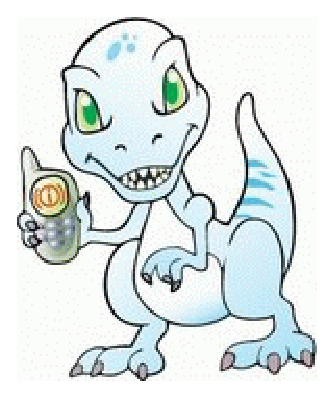
\includegraphics[width=4cm]{beestje.ps}
\end{center}
\FromSlide{3}
\begin{center}
\Red{Are you sure that you can trust these applications?}
\end{center}
\end{slide}
}

\begin{slide}{Security for trusted personal devices}
\begin{itemize}
\item \Blue{Trusted personal devices:} phones, smart cards, pda's, set
top boxes, \dots
\item Used for security-sensitive applications
\item Network connected
\item Support for complex applications (contain a full JVM)
\item Shift from hardware attacks to logical attacks
\end{itemize}
\end{slide}

\begin{slide}{Guaranteeing security}
\begin{itemize}
\item Formal specification and verification
\item Java Modeling Language (JML) able to express security properties
\item Classical program calculi can be used
\item Large body of theory on sound modular verification
\item Proof Carrying Code paradigm
\end{itemize}
\end{slide}

\overlays{5}{
\begin{slide}{But how to convince developers do this?}
\begin{itemstep}
\item Seamless integration in standard development environment
\item Small overhead in specification writing: annotation generation
\item Verification conditions automatically generated, proven by
automatic theorem prover
\item Reasoning at source code \emph{and} at bytecode level
\item Advanced support for difficult tasks (like interactive proving)
\end{itemstep}
\end{slide}
}

\begin{slide}{JACK: Java Applet Correctness Kit}
\vspace*{-1.5em}
\begin{center}
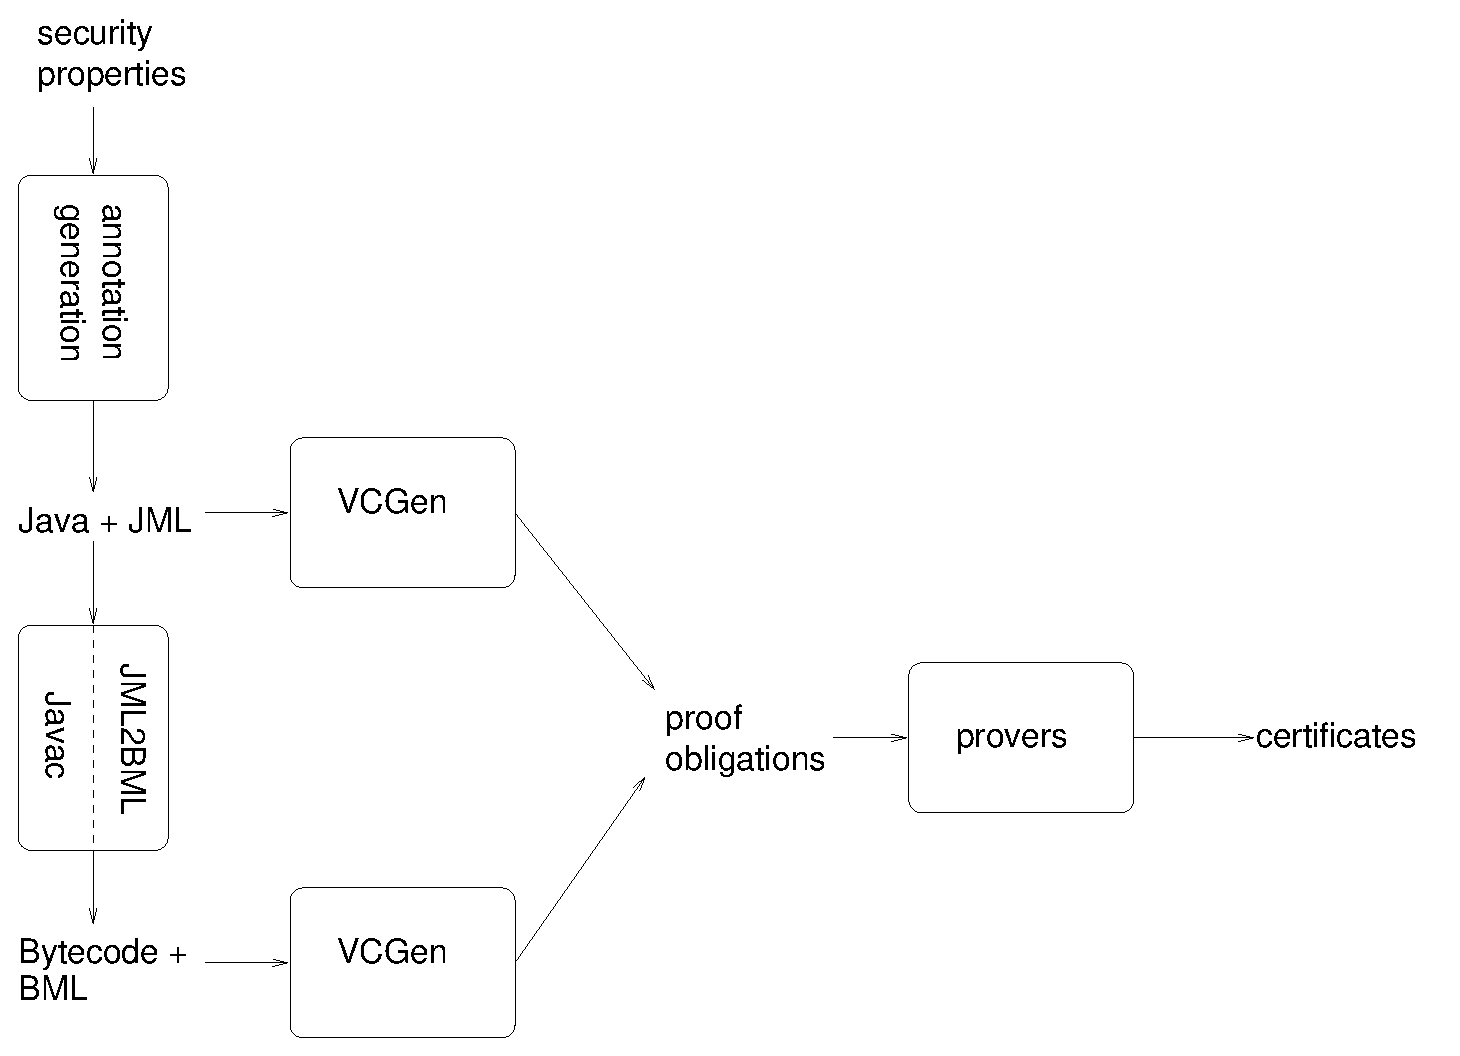
\includegraphics[height=\textheight]{toolset.eps}
\end{center}
\end{slide}

\begin{slide}{History of JACK}
\begin{itemize}
\item Development started at Gemplus (Jan 2002 to April 2003)\\
Objective: Give developers tools that help them to provide and be
accountable for a certain quality level of their code
\begin{itemize}
\item Conform to specification requirements
\item Well-documented
\item Without bugs
\end{itemize}
\item Transfered to INRIA (September 2003)
\begin{itemize}
\item Correctness stays major concern
\item More features \& plugins
\end{itemize}
\end{itemize}
\end{slide}

\begin{slide}{Features of JACK}
\begin{itemize}
\item Tight integration with IDE Eclipse
\item JML used as annotation language
\item Different means of validation possible

\item Special JACK view for verification condition browsing
\item Propagation of annotations, based on implementation of
verification condition generator
\end{itemize}
\end{slide}

\begin{slide}{And more features of JACK}
\begin{itemize}
\item JML specifications compiled into BML (Bytecode Modeling Language)
\item Support for verification of bytecode 
\item Support for Simplify (automatic) and Coq (interactive) prover
\end{itemize}
\end{slide}

\part{Integration with Eclipse}
\begin{slide}{Developing an application in Eclipse}
\vspace*{-1.5em}
\includegraphics[height=\textheight]{screen1.ps}
\end{slide}

\begin{slide}{Using Simplify}
\vspace*{-1.5em}
\includegraphics[height=\textheight]{screen2.ps}
\end{slide}

\begin{slide}{Proof obligation viewer}
\vspace*{-1.5em}
\includegraphics[height=\textheight]{screen3.ps}
\end{slide}

\begin{slide}{Reasoning with method calls}
\vspace*{-1.5em}
\includegraphics[height=\textheight]{screen4.ps}
\end{slide}

\begin{slide}{Reasoning about exceptions}
\vspace*{-1.5em}
\includegraphics[height=\textheight]{screen5.ps}
\end{slide}

\begin{slide}{Proof obligations}
\vspace*{-1.5em}
\includegraphics[height=\textheight]{screen6.ps}
\end{slide}

\begin{slide}{Proof obligations in Coq}
\vspace*{-1.5em}
\includegraphics[height=\textheight]{screen7.ps}
\end{slide}

\begin{slide}{Proof obligations in Simplify}
\vspace*{-1.5em}
\includegraphics[height=\textheight]{screen8.ps}
\end{slide}

\part{Annotation generation}

\begin{slide}{The cost of writing annotations}
\begin{itemize}
\item Annotation writing labour-intensive and error-prone
\item Much time spend on specifying obvious properties
\item Annotations for a simple security property often scattered
through the code
\item For static verification, method specifications need to be
relatively complete
\end{itemize}
\end{slide}

\begin{slide}{Runtime checking vs. static verification}
\begin{itemize}
\item Method \Blue{m} has specification: 
\Blue{requires P; ensures Q}
\item Method \Blue{n} calls method \Blue{m}\\
\item \Red{Runtime checking}: at all calls to \Blue{m} the specification is
tested
\item \Red{Static checking}: if \Blue{n} does not establish \Blue{P}, it
needs to be propagated\\ Specification for \Blue{n}:
\Blue{requires P}
\item If \Blue{n} does not invalidate \Blue{Q}, it can be
propagated
\end{itemize}
\end{slide}

\begin{slide}{Annotation generation in JACK}
\begin{itemize}
\item Precondition generation to avoid nullpointer exceptions and
array index out of bound exceptions
\item Assignable clause generation
\item Annotation generation to capture security properties, with
annotation propagation
\item Implementation uses weakest precondition implementation:
annotations are extracted from generated verification conditions
\end{itemize}
\end{slide}

\begin{slide}{Generation of preconditions and assignable clauses}
\includegraphics[width=\textwidth]{screen9.ps}
\end{slide}

\begin{slide}{Assertion generation}
Two phases:
\begin{itemize}
\item \Blue{synthesising} core-annotations
\item \Blue{weaving} annotations throughout the application
\end{itemize}
\ \smallskip\\
\Blue{Synthesising}: for each property annotations have to be defined
\bigskip\\
\Blue{Weaving}: algorithm for pre- and postcondition generation\\ \ \\
\end{slide}

\begin{slide}{Example core-annotations}
\Red{No nested transactions}
\begin{alltt}
\Blue{\textbf{/*@ static ghost int TRANSACT == 0; @*/}}
\end{alltt}
\ \smallskip\\
Method \textttbf{beginTransaction}
\begin{alltt}
\Blue{\textbf{/*@ requires TRANSACT == 0;
  @ assignable TRANSACT;
  @ ensures TRANSACT == 1; @*/}}
\textbf{public static native 
   void beginTransaction() 
        throws TransactionException;}
\end{alltt}
\ \smallskip\\
Similar annotations for \textttbf{commitTransaction},
\textttbf{abortTransaction} \\ \
\end{slide}


\begin{slide}{Preconditions for methods}
\begin{alltt}
\textbf{public void m() \{
   ...
   \Blue{// will require TRANSACT == 0}
   JCSystem.beginTransaction();
   \Blue{// TRANSACT modified} 
   \Blue{// ensures TRANSACT == 1}
   ...
   \Blue{// will require TRANSACT == 1}
   JSSystem.commitTransaction();
   \Blue{// TRANSACT modified} 
   \Blue{// ensures TRANSACT == 0}
   ...
   \}}
\end{alltt}
\end{slide}

\begin{slide}{Results}
\begin{itemize}
\item Tested on several realistic smart card applications
\item One core-annotation can give rise to many annotations in
different classes (26 annotations, spread over 5 different classes)
\item Several violations found: uncaught exceptions possible within
transactions 
\end{itemize}
\end{slide}

\begin{slide}{Uncaught exception within transaction}
\begin{alltt}
\textbf{void appExchangeCurrency(...) \{
   ...
   \Blue{/*@ exsures (Exception) TRANSACT == 0; @*/} \{
      ...
      JCSystem.beginTransaction();	
      try \{balance.setValue(decimal2);
            ...
      \} catch (DecimalException e) \{
         ISOException.throwIt(
              PurseApplet.OVERFLOW);
      \}
      JCSystem.commitTransaction();
   \}
   ...\}}
\end{alltt}
\end{slide}

\part{Support for bytecode}
\begin{slide}{Proof carrying code}
\begin{itemize}
\item Code producer 
 \begin{itemize}
 \item develops application and builds evidence for its correctness 
 \item ships application and evidence 
 \end{itemize}
\item Code client  
 \begin{itemize}
 \item generates verification conditions for the application
 \item checks that the evidence is a proof for the verification
conditions  
 \end{itemize}
\end{itemize}
\end{slide}

\begin{slide}{A framework for verification of bytecode}
 \begin{itemize}
 \item Bytecode Modeling Language (BML)
 \item Compiler from JML to BML
 \item Verification condition generator
 \item Equivalence with source code verification
 \end{itemize}
\end{slide}


\begin{slide}{BML}
 \begin{itemize}
 \item Follows closely the syntax and semantics of JML
 \item Expression language extended with bytecode specific constructs
(constant pool indexes, local variables, stack counter, stack 
expressions)
 \item Structural and type checking, \`a la BCV
 \item Encoding in class file format
  \begin{itemize}
   \item Java compiler independent 
   \item JVM compatibility: user-specific attributes, indexing to
relevant program point
   \item Efficiency of JVM not affected
  \end{itemize}
 \end{itemize}
\end{slide} 

\begin{slide}{Example: quicksort}
\vspace*{-1.5em}
\includegraphics[height=\textheight]{screen13.ps}
\end{slide}

\begin{slide}{Generated class file}
\vspace*{-1.5em}
\includegraphics[height=\textheight]{screen10.ps}
\end{slide}

\begin{slide}{Method specification in BML}
\vspace*{-1.5em}
\includegraphics[height=\textheight]{screen11.ps}
\end{slide}

\begin{slide}{Loop specification in BML}
\vspace*{-1.5em}
\includegraphics[height=\textheight]{screen12.ps}
\end{slide}





\begin{slide}{JML to BML compiler}
 \begin{itemize}
 \item Input:
 \begin{itemize}
  \item Source file annotated with JML 
  \item Corresponding class file, decorated with
\textbf{Local\_Variable\_Table} and \textbf{Line\_Number\_Table} 
 \end{itemize}
 \item Steps:
 \begin{itemize}
  \item Declarations of ghost and model fields
  \item Linking 
  \item Locating indexes for annotation statements
  \item Compilation of JML predicates
  \item Generation of user-specific class attributes
 \end{itemize}
 
\end{itemize}
\end{slide}

\begin{slide}{Verification condition generator}
\begin{itemize}
 \item Covers the most important feature of 
 Java - object manipulation and creation, exceptions, 
method invocations, arithmetic, stack manipulation etc.
 
 \item Contract-based approach
 \item Uses frame conditions for generation of tractable and provable
verification conditions
 \item Proven sound under the hypothesis that the control flow graph is reducible
\end{itemize}
\end{slide}

 
\begin{slide}{Relation between proof obligations on source and bytecode}
\begin{itemize}
\item Assumptions:
 \begin{itemize}
 \item non-optimising compiler 
 \item compiler produces reducible control flow graphs
 \item compiler preserves exception handling
 \end{itemize}

\item Equivalence proven modulo:
 \begin{itemize}
 \item names - Java names are compiled into indexes of the constant pool or elements in the method's local variable table
 
 \item types - Java types integer, short, byte and boolean are
 compiled into integers
 
 \end{itemize}
\end{itemize}
\end{slide}

\part{Support for interactive verification}

\begin{slide}{Specification and verification of complex properties}
\begin{itemize}
\item For complex properties, automatic verification often not
sufficient 
\item Such properties often use advanced specification techniques
(JML model features)
\item Interactive prover support necessary: \Blue{Coq}
\item Introduction of \Blue{native} construct to bridge gap between
JML models and logic of theorem prover
\end{itemize}
\end{slide}

\begin{slide}{Coq}
\begin{itemize}
\item Based on \Blue{calculus of inductive constructions}
\item Can express types, axioms, functions, variables, definitions,
lemmas \dots
\item Lemmas have to be proved, by building \Blue{proof term} out of
the types, axioms, variables etc.
\item \Blue{Tactics}: special commands called within a proof script
\item \Blue{Custom tactics} can be created from more primitive ones
\item Coq can easily express the logics for Jack
\end{itemize}
\end{slide}


\begin{slide}{POs generated by Jack}
\begin{itemize}
\item Each hypothesis comes with \Blue{hints} about its origin
\begin{itemize}
\item Useful information for proof script 
\item Separation of hypotheses
\item Nearly human readable
\end{itemize}
\item Uses Coq's \Blue{pretty printing} 
\item Tactics for cleaning and proving
\begin{itemize}
\item Achieves some level of automation
\item Simplify is better for automatic proving
\item But Coq proves (interactively) proof obligations that Simplify
cannot handle
\end{itemize}
\end{itemize}
\end{slide} 

\begin{slide}{ProverEditor}
\begin{itemize}
\item \Blue{Syntax highlighting}
 for both Coq file and proof view window
\item Same \Blue{keyboard shortcuts} as CoqIde
\item Full integration within Eclipse
  \begin{itemize}
  \item No weird pop-up except if user wants to use another editor
  \item Management of proof files is easier
  \end{itemize}
  
\item Also usable with ESC/Java
\item Handles of \Blue{large} files ($>$ 1 Mo)
\end{itemize}
\end{slide}

\begin{slide}{What it looks like}
\vspace*{-1.5em}
\begin{center}
\includegraphics[height=\textheight]{screen14.ps}
\end{center}
\end{slide}

\overlays{2}{
\begin{slide}{Specifications of complex properties: use of pure methods}
\begin{itemize}
\item A method is \Blue{pure} when it has no visible side effect
\item Pure methods can be used in specifications
%\begin{tabbing}
% /*\=@ \Blue{requires} true;\+\\
%   @ \Blue{ensures} $\backslash$result == ((tab != null) \&\& (i $>=$ 0) \&\& (i $<$ tab.length));\\
%   @*/\-\\
% public\= /*@ \Blue{pure} @*/ boolean withinBounds(Object[] tab, int i) \{\\
% 	\>return (tab != null) \&\& (i $>=$ 0) \&\& (i $<$ tab.length);\\
% \}\\
% \end{tabbing}
\item \Blue{Model methods} are pure methods that exist only for
specifications 
\item Complicates verification: specification of pure method has to be
used 
\item Our approach: define the pure method in Coq in directly
\end{itemize}
\FromSlide{2}
\begin{center}
\Blue{Native specifications}
\end{center}
\end{slide}
}



\begin{slide}{Native methods}
\begin{itemize}
\item In JML:
\begin{alltt}
//@ public \Blue{native} boolean 
       withinBounds(Object[] tab, int i);
\end{alltt}
\item In the Coq file user\_extensions.v:
\begin{alltt}
\Blue{Definition} withinBounds : 
  Reference \(\rightarrow\) 
  (Reference \(\rightarrow\) t\_int \(\rightarrow\) Reference)\(\rightarrow\)  
  t\_int \(\rightarrow\) bool := 
\Blue{fun} tab intelements value \Blue{=>} 
    and (tab != null) (and (0 <= value) 
    (value < (arraylength tab))).
\end{alltt}
\end{itemize}
\end{slide}

\begin{slide}{Native types}
\begin{itemize}
\item To express complex properties, advanced datatypes useful
\item Easily defined in Coq, not in JML
\item \Blue{Native types}: \\
Coq types in JML: 
\begin{alltt}
//@  public \Blue{native} class ObjectSet; 
\end{alltt}
In the Coq file user\_extensions.v:
\begin{alltt}
  \Blue{Definition} ObjectSet : set Reference.
\end{alltt}
\end{itemize}
\end{slide}

\begin{slide}{What are native types?}
\begin{itemize}
\item Native types are not standard Java/JML class types:
\begin{itemize}
\item Do not inherit from Object
\item No constructors
\item No casts
\item No instance creation
\end{itemize}
\item Native types are \Blue{functional type}: 
\begin{itemize}
\item Modifiers are `static'
\item Modifiers create new objects 
\end{itemize}
\end{itemize}
\end{slide}

\begin{slide}{Example: set library}
We can define a Coq set library to use in annotations\\

In JML we \Blue{declare}:
\begin{alltt}
/*@ public native class ObjectSet \{
  @ public native static ObjectSet 
              \Blue{create}();
  @ public native static ObjectSet 
  @           \Blue{add}(ObjectSet os, Object o);
  @ public native boolean 
              \Blue{member}(Object o);
  @ public static native ObjectSet 
  @           \Blue{toSet}(Object [] tab);
  @ \}
  @*/
\end{alltt}
\end{slide}

\begin{slide}{Example: set library}
In Coq we \Blue{define}:
\begin{alltt}
Definition \Blue{ObjectSet} := set Reference. 
Definition \Blue{ObjectSet\_create} := 
                     empty\_set.
Definition \Blue{ObjectSet\_add} 
                     (os: ObjectSet) 
                     (o: Reference) :=  
                     set\_add o os.
Definition \Blue{ObjectSet\_member} 
                     (this: ObjectSet) 
                     (o: Reference) := 
                     set\_mem o this
\end{alltt}
\end{slide}

\begin{slide}{To conclude...}
\end{slide}
\end{document}
